\begin{frame}[fragile]
  \frametitle{CUDA programming: Lab 4: intrinsics, streams, tools}
\begin{itemize}
\item In this lab we shall learn about \mydef{CUDA math library}, \mydef{streams}, \mydef{nsight} tools
\item Let us create on CPU a big array, initialize it with random numbers, copy it to GPU, apply some math functions to it and copy it back to the host.
\item Here is the kernel
{\tiny
{\color{mycolorcode}
\begin{verbatim}
__global__ void map(float *d_a, int n, int m)
{
  int id = blockDim.x * blockIdx.x  + threadIdx.x;
  
  if(id < n)
    for(int i = 0; i < m; ++i)
      {
        d_a[id] = sinf(d_a[id]) + cosf(d_a[id]);
        d_a[id] = expf(d_a[id]);
        d_a[id] = rsqrtf(d_a[id]) - d_a[id];
      }
}
\end{verbatim}
}
}
\item In CUDA there are \mydef{standard math functions} - can be executed both on the host and device -  and \mydef{intrinsic functions} - can only run on device, are faster but less precise.
\item The code above uses standard functions.
\end{itemize}
\end{frame}

\begin{frame}[fragile]
  \frametitle{CUDA programming: Lab 4: intrinsics, streams, tools}
\begin{itemize}
\item Examples of standard math functions: \mycode{sqrtf}, \mycode{sqrt}, \mycode{rsqrtf}, \mycode{rsqrt}, \mycode{sinf}, \mycode{sin}, etc. Those are single and double precision functions.
\item Examples of the corresponding intrisic functions: {\color{mycolorcode}\verb|__fsqrt_rn|}, {\color{mycolorcode}\verb|__frsqrt_rn|}, {\color{mycolorcode}\verb|__sinf|}, etc. The precision is less than float.
\item If one can afford less accurate functions, one can either replace the functions in the code or use compile option {\color{mycolorcli}\verb|--use_fast_math|} to replace all the standard functions by the corresponding intrinsic 
  functions.
\item Let us measure the performance of the same kernel with standard and intrinsic math functions: 131 vs 27 ms! This kernel runs almost 5 times faster with intrinsic functions than with standard ones.
\item Let us look how the results are different:
{\tiny
{\color{mycolorcli}
\begin{verbatim}
a[0] = 1.74003, a[1] = 1.45576, a[2] = -3.50318, a[3] = -3.0294, a[4] = -3.22013 ...
vs
a[0] = 1.74017, a[1] = 1.45575, a[2] = -3.50318, a[3] = -3.02938, a[4] = -3.22022 ...
\end{verbatim}
}
}
\item Not a big difference in numerical results.
\item Consult the tables in the ``CUDA C Programming Guide'' for precision guarantees and the complete list of the available functions.
\end{itemize}
\end{frame}


\begin{frame}[fragile]
  \frametitle{CUDA programming: Lab 4: intrinsics, streams, tools}
\begin{itemize}
\item Let us run the program through \mydef{nvvp profiler}
\item We see that first the program spends significant time transfering data from host to device, then comparable amount of time is spent on the computations and transfering the results back to the host.
\end{itemize}
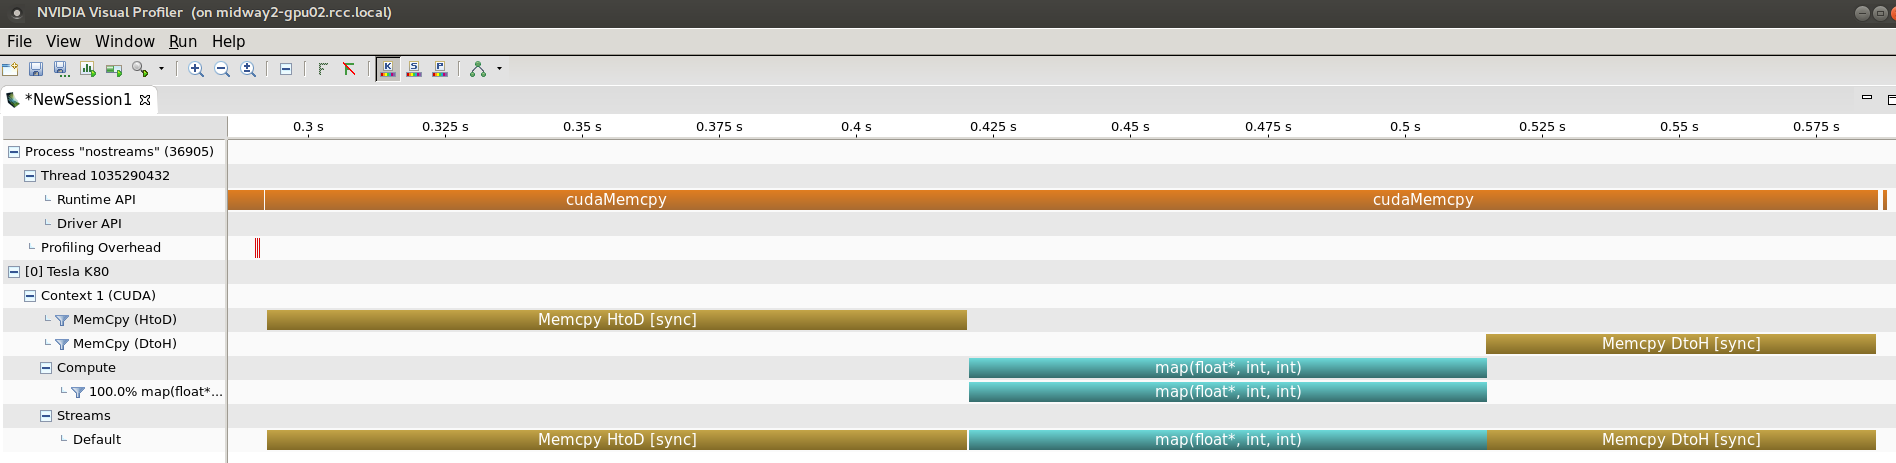
\includegraphics[width=11.9cm]{graphs/nostreams.png}
\begin{itemize}
\item Meanwhile, the computations are embarrasingly parallel and independent for each element of the array.
\item Would not it be better first to transfer a part of data, start computations on GPU on the first part of the data, transfer in parallel with the computations second part, etc. to hide the latency
\end{itemize}
\end{frame}

\begin{frame}[fragile]
  \frametitle{CUDA programming: Lab 4: intrinsics, streams, tools}
\begin{itemize}
\item Some devices of compute capability 2.x and higher can execute multiple
kernels concurrently. Applications may query this capability by checking the
\mycli{concurrentKernels} device property, which is equal to 1 for
devices that support it.
\item The maximum number of kernel launches that a device can execute concurrently
depends on its compute capability.
\item Some devices can perform an asynchronous memory copy to or from the GPU
concurrently with kernel execution. Applications may query this capability by checking
the \mycli{asyncEngineCount} device property, which is greater
than zero for devices that support it. If host memory is involved in the copy, it must be
page-locked
\item Some devices of compute capability 2.x and higher can overlap copies to and from the
device. Applications may query this capability by checking the \mycli{asyncEngineCount}
device property, which is equal to 2 for devices that support
it. In order to be overlapped, any host memory involved in the transfers must be page-locked.

\end{itemize}
\end{frame}


\begin{frame}[fragile]
  \frametitle{CUDA programming: Lab 4: intrinsics, streams, tools}
\begin{itemize}
\item For K80, according to \mycli{deviceQuery} from Lab 1:
{\tiny
{\color{mycolorcli}
\begin{verbatim}
Concurrent copy and kernel execution:  Yes with 2 copy engine(s)
\end{verbatim}
}
}
\item CUDA construction that can help to interleave computations and data transfer is called \mydef{streams}
\item A stream is a sequence of commands (possibly issued by different host threads) that
execute in order. Different streams, on the other hand, may execute their commands out
of order with respect to one another or concurrently.
\item A stream is defined by creating a stream object and specifying it as the stream parameter
to a sequence of kernel launches and host to/from device memory copies.
\item To use streams for data transfer between host and device, one needs to allocated memory on the host not with \mycode{malloc} but as follows
{\color{mycolorcode}
\begin{verbatim}
 float *h_a = NULL;
  cudaMallocHost(&h_a, size);
\end{verbatim}
}
to ensure that the memory allocated on the host is \mydef{page-locked} (cannot be swapped)
\end{itemize}
\end{frame}


\begin{frame}[fragile]
  \frametitle{CUDA programming: Lab 4: intrinsics, streams, tools}
\begin{itemize}
\item Next we need to create streams:
{\color{mycolorcode}
\begin{verbatim}
cudaStream_t stream[nstreams];
for(int i = 0; i < nstreams; ++i)
  cudaStreamCreate(&stream[i]);
\end{verbatim}
}
\item Send data between host and device in batches and run a kernel on each batch to interleave computations and data transfer:
{\tiny
{\color{mycolorcode}
\begin{verbatim}
for(int i = 0; i < nstreams; ++i)
{
  cudaMemcpyAsync(d_a + i*batch, h_a + i*batch, batch_size, cudaMemcpyHostToDevice, stream[i]);
  map<<<grid_size, block_size, 0, stream[i]>>>(d_a + i*batch, batch, iterations)
  cudaMemcpyAsync(h_a + i*batch, d_a + i*batch, batch_size, cudaMemcpyDeviceToHost, stream[i]);
}
\end{verbatim}
}
}
\item Notice: we provide \mycode{stream[i]} argument to data transfer operations and to a kernel call.
\item Also note: instead of \mycode{cudaMemcpy} we use asynchronous version \mycode{cudaMemcpyAsync} that, contrary to \mycode{cudaMemcpy} immediately returns without waiting for data transfer to finish.
\end{itemize}
\end{frame}

\begin{frame}[fragile]
  \frametitle{CUDA programming: Lab 4: intrinsics, streams, tools}
\begin{itemize}
\item To free resources, we need to destroy streams and release page-locked memory (not with \mycode{free} but with \mycode{cudaFreeHost}):
{\color{mycolorcode}
\begin{verbatim}
for(int i = 0; i < nstreams; ++i)
  cudaStreamDestroy(streams[i])
cudaFreeHost(h_a);
\end{verbatim}
}
\item In case the device is still doing work in the stream when \mycode{cudaStreamDestroy()} is
called, the function will return immediately and the resources associated with the stream
will be released automatically once the device has completed all work in the stream.
\item Kernel launches and host to/from device memory copies that do not specify any stream
parameter, or equivalently that set the stream parameter to zero, are issued to the default
stream. They are therefore executed in order.
\end{itemize}
\end{frame}


\begin{frame}[fragile]
  \frametitle{CUDA programming: Lab 4: intrinsics, streams, tools}
\begin{itemize}
\item Let us now run nvvp and see if we succeeded in interleaving data transfer and computations:
\end{itemize}
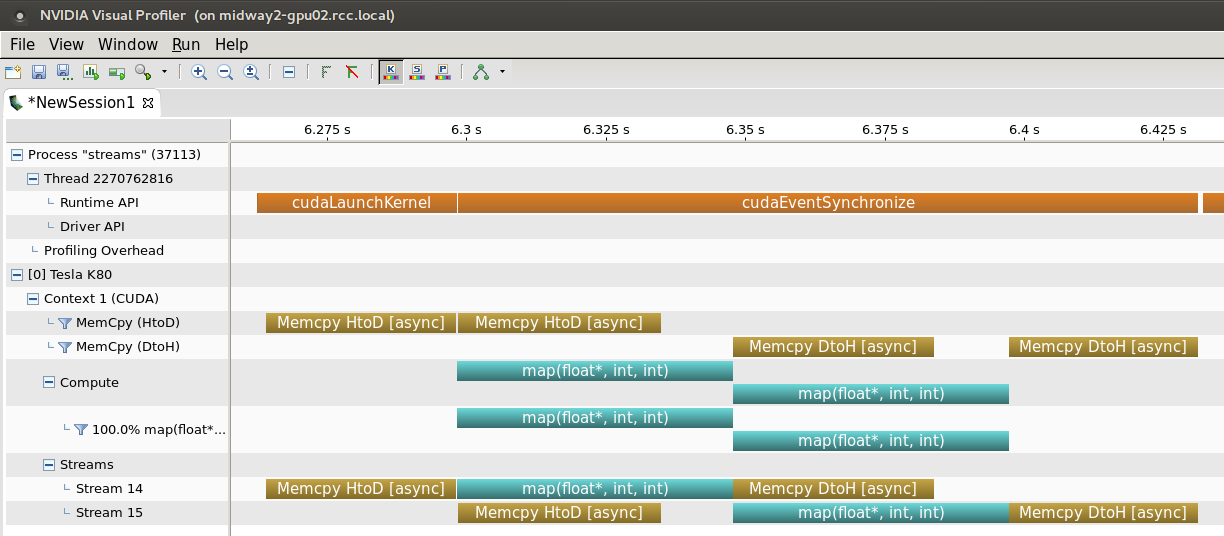
\includegraphics[width=11.9cm]{graphs/streams.png}
\end{frame}

\begin{frame}[fragile]
  \frametitle{CUDA programming: Lab 4: intrinsics, streams, tools}
\begin{itemize}
\item As you can see, kernel and data transfer are indeed interleaved but only one kernel runs at a time. This is probably the limitation of K80.
\item Let us see how it affected timing: 223 ms vs 138 ms.
\item Newer GPU cards might benefit more from streams.
\item There are various ways to explicitly synchronize streams with each other:
  \begin{itemize}
  \item \mycode{cudaDeviceSynchronize()} waits until all preceding commands in all streams of all
    host threads have completed.
  \item \mycode{cudaStreamSynchronize()} takes a stream as a parameter and waits until all preceding
    commands in the given stream have completed. It can be used to synchronize the host
    with a specific stream, allowing other streams to continue executing on the device.
  \item \mycode{cudaStreamWaitEvent()} takes a stream and an event as parameters and makes all the commands added to the given stream after
    the call to \mycode{cudaStreamWaitEvent()} delay their execution until the given event has
    completed. The stream can be 0, in which case all the commands added to any stream
    after the call to \mycode{cudaStreamWaitEvent()} wait on the event.
  \end{itemize}
\end{itemize}
\end{frame}

\begin{frame}[fragile]
  \frametitle{CUDA programming: Lab 4: intrinsics, streams, tools}
\begin{itemize}
\item More ways to explicitly synchronize streams with each other.
  \begin{itemize}
  \item \mycode{cudaStreamQuery()} provides applications with a way to know if all preceding
    commands in a stream have completed
  \end{itemize}
  \item One can insert a \mydef{callback} at any point into a stream via
    \mycode{cudaStreamAddCallback()}. A callback is a function that is executed on the host once
    all commands issued to the stream before the callback have completed. Callbacks in
    stream 0 are executed once all preceding tasks and commands issued in all streams
    before the callback have completed.
  \item The relative priorities of streams can be specified at creation using
    \mycode{cudaStreamCreateWithPriority()}.
\end{itemize}
\end{frame}

\begin{frame}[fragile]
  \frametitle{CUDA programming: Lab 4: intrinsics, streams, tools}
\begin{itemize}
  \item Instead of specifying what tasks run in what streams and what are dependencies between the tasks, one can use \mydef{graphs}
  \item Graphs present a new model for work submission in CUDA. A graph is a series of
    operations, such as kernel launches, connected by dependencies, which is defined
    separately from its execution. 
  \item This allows a graph to be defined once and then launched
    repeatedly. 
  \item Separating out the definition of a graph from its execution enables a number
    of optimizations: first, CPU launch costs are reduced compared to streams, because
    much of the setup is done in advance; second, presenting the whole workflow to CUDA
    enables optimizations which might not be possible with the piecewise work submission
    mechanism of streams.
  \item Graphs can be created with Graph API or by capturing an old fashioned streams based program.
\end{itemize}
\end{frame}


\begin{frame}[fragile]
  \frametitle{CUDA programming: Lab 4: intrinsics, streams, tools}
\begin{itemize}
\item As was mentioned before, to interleave data transfer and computations, the corresponding part of the host memory should be \mydef{pinned} or \mydef{page-locked}.
\item That means that it cannot be swapped to disk by OS.
\item Other uses of pinned memory:
  \begin{itemize}
  \item On some devices, page-locked host memory can be mapped into the address space
    of the device, eliminating the need to copy it to or from device memory
  \item On some systems bandwidth between host memory and device
    memory is higher if host memory is allocated as page-locked
  \end{itemize}
\item However, page-locked host memory is a scarce resource, so allocations in page-locked
  memory will start failing long before allocations in pageable memory. In addition, by
  reducing the amount of physical memory available to the operating system for paging,
  consuming too much page-locked memory reduces overall system performance.
\end{itemize}
\end{frame}

\begin{frame}[fragile]
  \frametitle{CUDA programming: Lab 4: intrinsics, streams, tools}
\begin{itemize}
\item We have already seen \mycli{nvvp} profiler.
\item CUDA comes with a suite of tools for debugging and profiling:
  \begin{itemize}
  \item There IDE with debugger, profiler, editor called \mycli{nsight}
  \item For \mycli{nsight} to show the source code, you need to compile it with \mycli{-g -G} option to \mycli{nvcc}
  \item Instead of using \mycli{nsight} GUI, you can run cli-based \mycli{cuda-gdb} which has similar interface as \mycli{gdb}. It allows to look into each thread separately.
  \item \mycli{cuda-memcheck} can be used to diagnose memory problems
  \item If you cannot run profiler on the node interactively, you can run it as a batch job and then look at the results with GUI.
  \item You can also run \mycli{nsight} remotely
  \end{itemize}
\item \mycli{nsight} is supposed to be deprecated soon and replaced by \mycli{nsight compute} and \mycli{nsight systems}. So far I can run those on my laptop (Ubuntu 16.04) but not on midway (Scientific Linux 7): they seem to require newer version of \mycli{glibc}.
\end{itemize}
\end{frame}


\begin{frame}[fragile]
  \frametitle{CUDA programming: Lab 4: intrinsics, streams, tools}
\begin{itemize}
\item We have already seen how to use \mydef{events} to time program execution.
\item CUDA lets the application asynchronously record events at
  any point in the program and query when these events are completed. 
\item An event has completed when all tasks - or optionally, all commands in a given stream - preceding the
  event have completed. 
\item Events in stream zero are completed after all preceding tasks and
  commands in all streams are completed.
\end{itemize}
{\small
{\color{mycolorcode}
\begin{verbatim}
cudaEvent_t start, stop;
cudaEventCreate(&start); cudaEventCreate(&stop);
cudaEventRecord(start);
map<<<grid_size, block_size>>>(d_a, N, iterations);
cudaEventRecord(stop); 
cudaEventSynchronize(stop);
cudaEventElapsedTime(&milliseconds, start, stop);
cudaEventDestroy(start); cudaEventDestroy(stop);
\end{verbatim}
}
}
\end{frame}
